\documentclass[13pt,oneside]{book}
\usepackage[utf8]{inputenc}
\usepackage{url}
\usepackage{listings}
\usepackage{graphicx}

\usepackage{geometry}
\geometry{a4paper, left=20mm, right=20mm, top=20mm, bottom=20mm}
\usepackage[toc,page]{appendix}
\usepackage{graphicx}
\usepackage{natbib}
\usepackage{caption}

\begin{document}

\captionsetup[figure]{margin=1.5cm,font=small,labelfont={bf},name={Figure},labelsep=colon,textfont={it}}
\captionsetup[table]{margin=1.5cm,font=small,labelfont={bf},name={Table},labelsep=colon,textfont={it}}


\begin{titlepage}
\begin{center}
{\LARGE College Of Engineering Trivandrum}\\[3cm]
\linespread{1.2}\huge {\bfseries System Software Lab}\\[3cm]
\linespread{1}

\includegraphics[width=5cm]{img/emblem.jpeg}\\[3cm]
{\Large GOKUL K\\ S5  CSE \\ Roll No:21\\ TVE18CS021 }\\[1cm]


\textit{ }\\[2cm]
Department of Computer Science\\[0.2cm]
\today
\end{center}

\end{titlepage}

\newpage

\begin{frame}{}
    \centering
    \hspace*{-0.5cm}
    $\vcenter{\hbox{
\includegraphics[width=1.5cm]{img/emblem.jpeg}}}$
    $\vcenter{\resizebox{0.95\textwidth}{!}{
        \begin{tabular}{c}
             CS331 - System Software Lab $\cdot$ 2020 $\cdot$   \\
             \hline 
        \end{tabular}
    }}$
\end{frame}
\section*{Cycle 2}
\section*{Expt 8}
\begin{center}
    \Large{Pass 1 of a two pass assembler}
\end{center}
\section*{Aim}
\large
Implement pass one of a two pass assembler

\section*{Algorithm} 
    \begin{verbatim}
1 begin
2 read first input line
3 if OPCODE = ’START ’ then
4 begin
5 save #[ OPERAND ] as starting address
6 initialized LOCCTR to starting address
7 write line to intermediate file
8 read next input line
9 end {if START }
10 else
11 initialized LOCCTR to 0
12 while OPCODE != ’END ’ do
13 begin
14 if this is not a comment line then
15 begin
16 if there is a symbol in the LABEL field then
17 begin
18 search SYMTAB for LABEL
19 if found then
20 set error flag ( duplicate symbol )
21 else
22 insert ( LABEL , LOCCTR ) into SYMTAB
23 end {if symbol }
24 search OPTAB for OPCODE
25 if found then
26 add 3 { instruction lengh } to LOCCTR
27 else if OPCODE = ’WORD ’ then
28 add 3 to LOCCTR
29 else if OPCODE = ’RESW ’ then
30 add 3 * #[ OPERAND ] to LOCCTR
31 else if OPCODE = ’RESB ’ then
32 add #[ OPERAND ] to LOCCTR
33 else if OPCODE = ’BYTE ’ then
34 begin
35 find length of constant in bytes
36 add length to LOCCTR
37 end {if BYTE }
38 else
39 set error flag ( invalid operation code )
40 end {if not a comment }
41 write line to intermediate file
42 read next input line
43 end { while not END }
44 write last line to intermediate file
45 save ( LOCCTR - starting address ) as program length
46 end
	\end{verbatim}

\section*{Source Code}
\small

\begin{lstlisting}[language=C]
/* Implement pass one of a two pass assembler */

    \end{lstlisting}
    \begin{verbatim}
input.txt

COPY START 1000
** LDA ALPHA
** ADD ONE
** SUB TWO
** STA BETA
ALPHA BYTE C'KLNCE
ONE RESB 2
TWO WORD 5
BETA RESW 1
** END **
    
optab.txt
LDA 00
STA 23
ADD 01
SUB 05
\end{verbatim}
\section*{Output}
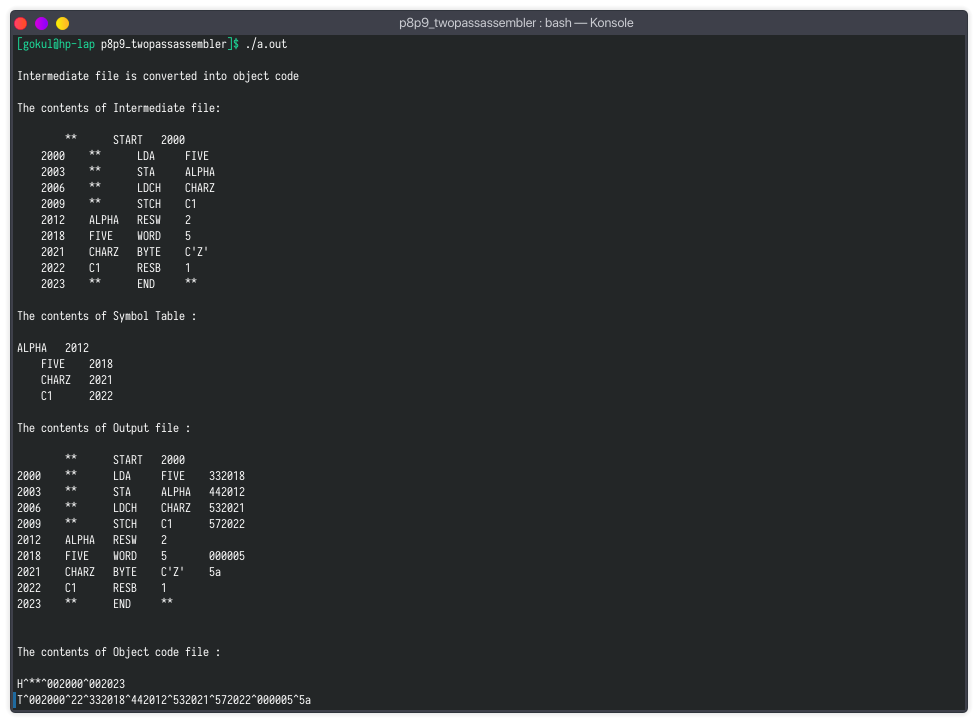
\includegraphics[width=\textwidth]{img/p8.png}
    
\Large
\section*{Result}
\large
The pass one of a two pass assembler was implemented and its output verified
\end{document}